\section{Original Method}
\label{sec:original}
The hybrid traffic signal controller (HTSC) of \cite{ref_paper} controls one isolated intersection and consists of four modules
(Fig.~\ref{fig:arch}).

\begin{figure}[t]
\centering
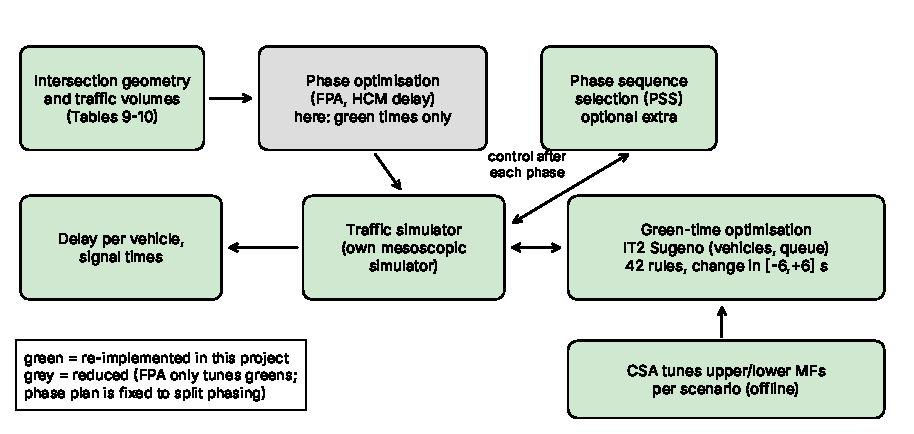
\includegraphics[width=0.92\linewidth]{fig_architecture.pdf}
\caption{Architecture of the reference HTSC (left) and the parts re-implemented in this project (grey box: reduced to FPA green-time tuning with a fixed split-phase plan).}\label{fig:arch}
\end{figure}

\textbf{Phase optimisation (FPA).} For a given geometry and demand, FPA searches the green times of all candidate phase plans (2, 3 or 4 phases),
using the flow-weighted HCM delay as objective, with $8\le g_i\le 60$~s, a degree-of-saturation limit $X\le1.4$, and a safety rule that allows a
permitted left turn only if (left-turn volume) $\times$ (conflicting volume) $<50\,000$. The plan with the lowest delay and its cycle length are kept;
the module is re-run every three cycles.

\textbf{Signal timing optimisation (interval Type-2 Sugeno).} At the end of every phase the controller reads two detector values for the
\emph{next} phase and returns a green-time change in $[-6,+6]$~s. The inputs are the number of vehicles in the 175~m detector range
(universe 0--40, 7 MFs) and the queue length (universe 0--175~m, 6 MFs); this gives $7\times6=42$ rules. The output has seven singletons
($-6,-4,\dots,+6$~s, Table~8 of the paper). The $\pm6$~s interval was selected by trying $\pm4$, $\pm6$, $\pm8$ and $\pm10$~s and an ANOVA
(Tables~6--7 of the paper). The centres and legs of the upper and lower triangular MFs are tuned by CSA, separately for each traffic scenario, with the
objective of minimum delay (Table~5 of the paper).

\textbf{Phase sequence selection.} Among the phases not yet served in the cycle, the one with most vehicles is served first.

\textbf{Experiments.} The system is evaluated in the authors' simulator KU-Trsim (exponential arrivals, Greenshields speed--density relation,
five vehicle types, 900~s runs) on four geometries (3-leg and 4-leg, each with and without left-turn pocket) and nine demand scenarios
(Tables~9--10), averaging 20 random seeds. Competitors are a fixed-time controller, FPA-TSC (phase optimisation only) and a Type-1 fuzzy controller
tuned with DE \cite{dogan2016}. Performance is the mean delay per vehicle, compared with the mean percentage error (MPE, Eq.~11 of the paper) and a Friedman test.
Reported improvements of HTSC over fixed time range from 11.6\% (3-leg) to 31.5\% (3-leg with pocket) (Table~13 of the paper).

\subsection*{Critical reading of the paper}
The following points were noted while reading and are taken into account in this study.
\begin{itemize}\setlength\itemsep{0pt}
\item The rule table, the height of the lower MFs, the population size of CSA and the training/evaluation seed policy are not stated, so exact replication is impossible. It is not stated whether the MFs were tuned and evaluated on the same simulation seeds, which would favour the tuned system.
\item The abstract's ``about 32\%'' improvement equals the best case in Table~13; the mean over the four geometries is lower (about 23.5\% when the four HTSC-versus-fixed entries are averaged). The ``approximately 60\%'' in the conclusions is derived from Friedman ranks, which are not percentages of delay.
\item Eq.~11 as printed gives positive values for an improvement, whereas Table~13 prints negative values; the caption of Fig.~16 says ``three-leg'' for a four-leg figure.
\item Table~7 does not label whether 0.992 is the Levene statistic or its $p$-value, and the ANOVA on $\pm4\dots\pm10$ pools six very different scenarios per group, so a non-significant $F$ cannot be read as equality of the intervals.
\item The Friedman test uses the nine scenarios per geometry as blocks; these are not independent random samples, so the $p$-values describe these nine cases only.
\item The advantage of Type-2 over Type-1 comes from a comparison in which the two systems differ in structure, optimiser (CSA versus DE) and phase optimisation, so the contribution of Type-2 alone is not isolated.
\item High demand saturates the intersection and all controllers approach fixed time; computing time of the optimisers is discussed qualitatively but not measured.
\end{itemize}

\section{Reproduction Methodology}
\label{sec:repro}
Because the reference simulator and code are unavailable, the minimum reproduction requirement (MRR) fixed for this project is the
\textbf{Type-1 and interval Type-2 Sugeno green-time controller with CSA-tuned MFs, evaluated on the 18 demand scenarios of the 3-leg and 4-leg geometries}, compared with
fixed-time and FPA-optimised fixed-time control. All code was written for this project with the help of an AI assistant (see the Generative AI Usage Disclosure); no code of the authors was used. Table~\ref{tab:diff} lists how the
re-implementation differs from the paper; these differences are the main reason why absolute delays cannot be compared with the paper.

\begin{table}[t]
\centering\small
\caption{Differences between the reference study and this re-implementation.}\label{tab:diff}
\begin{tabular}{@{}p{3.2cm}p{5.4cm}p{5.6cm}@{}}
\toprule
Aspect & Reference paper & This project \\ \midrule
Simulator & KU-Trsim, microscopic, acceleration tables & event-based mesoscopic, saturation headway $2.0\times$ vehicle factor (assumed) \\
Phase plan & FPA chooses 2/3/4-phase plan & split phasing (one phase per leg); FPA only tunes greens \\
Geometries & 3-leg, 4-leg, each $\pm$ left-turn pocket & 3-leg and 4-leg (no pocket variants) \\
Rule table & not published & monotone table of 42 rules (own design, Eq.~\eqref{eq:rule}) \\
Lower MF & read from figures & same apex, narrower legs, height 0.5 (assumed) \\
CSA budget & 2000 iterations, population not stated & 20 crows $\times$ 100 iterations, tuned on 4 seeds \\
Evaluation & 20 seeds (tuning seeds not stated) & 20 \emph{different} seeds, common random numbers \\
Type-1 baseline & DE-tuned FL \cite{dogan2016} & same structure and same CSA tuning as the Type-2 system \\
Phase sequence & used in HTSC & optional (reported as an extra row) \\ \bottomrule
\end{tabular}
\end{table}

\textbf{Simulator.} Vehicles of five types (80/10/5/3/2\%, lengths from Table~2 of the paper) arrive with exponential headways, are assigned to one of two lanes
and traverse the 175~m detector range at 50~km/h. A queue discharges with start-up lost time 3.6~s and a headway of 2.0~s multiplied by a vehicle factor
(1.0/1.15/1.8/2.0/1.6 for car/minibus/bus/lorry/truck, assumed because the Synchro acceleration tables are not reproduced); yellow is 2~s (vehicles may still cross) and all-red 1~s.
Delay is the time lost against free flow; vehicles still queued at 900~s are counted until 900~s. The simulator was validated against the HCM
delay model for fixed-time control (Section~\ref{sec:results}).

\textbf{Fuzzy controllers.} The rule table is a monotone design: for count MF $i\in\{0..6\}$ and queue MF $j\in\{0..5\}$ the consequent index is
\begin{equation}\label{eq:rule}
k_{ij}=\operatorname{round}\!\Big[3\Big(\tfrac{i}{6}+\tfrac{j}{5}\Big)\Big],\qquad z_{ij}=-6+2k_{ij}\ \text{s},
\end{equation}
so the green is shortened when few vehicles wait and extended when many do. The base green times are those found by FPA with the HCM objective (Eq.~7--9 of the paper) and
$8\le g\le60$~s; after the fuzzy change the green is clipped to $[5,66]$~s. A Type-1 and an interval Type-2 version share the same structure; the Type-2 version has an additional lower MF per set.

\textbf{MF encoding and tuning.} For each input variable the $K$ apexes (sorted), left legs and right legs are encoded in $[0,1]$ ($3K$ values, Type-1: 39 parameters in total); the Type-2 system adds two
lower-leg fractions per MF ($5K$ values, 65 parameters in total). The CSA population is initialised around the uniformly spaced MFs (first crow equal to them), so the tuned system can never be worse than the uniform design on the tuning seeds.
Fitness is the mean delay on four tuning seeds (1001--1004); the reported delays use 20 disjoint seeds (1--20) and the same demand realisations for every controller.

\section{Proposed Extension}
\label{sec:extension}
The extension is designed to test claims that the paper makes but does not isolate. All three parts use the controllers of Section~\ref{sec:repro}.

\textbf{A -- Optimiser comparison (technical rationale: the paper chooses CSA because it is fast, but never compares it with other optimisers on this task).}
CSA, FPA, PSO and DE tune the 65 parameters of the Type-2 system for each of the 18 scenarios, three independent runs each, with an identical budget of
$20\times61=1220$ simulation evaluations per run. Reported: delay reduction relative to the uniform-MF system on the test seeds, ranks, Friedman test and Holm-corrected Wilcoxon tests of CSA against the others,
and convergence curves.

\textbf{B -- Detector-noise robustness (rationale: the footprint of uncertainty is argued to make Type-2 less sensitive to measurement errors).}
The MFs tuned without noise are used unchanged; multiplicative Gaussian noise with standard deviation $\sigma\in\{0,10,20,30,50,75\}\%$ is applied to both inputs at every decision.
Hypothesis $H_1$: the loss of benefit relative to fixed time grows more slowly for Type-2 than for Type-1.

\textbf{C -- Type reduction and cost (rationale: engineering value).} The same Type-2 MFs are evaluated with Karnik--Mendel and with Nie--Tan type reduction (does the cheaper method change delay?),
and the inference time per decision and per 900~s simulation are measured. A supplementary \emph{budget study} runs Type-1 and Type-2 tuning with 400 instead of 100 iterations on four scenarios to see whether the
larger parameter space of Type-2 simply needs more search.

\section{Experimental Setup}
\label{sec:setup}
\begin{itemize}\setlength\itemsep{0pt}
\item \textbf{Software:} Python 3.13, NumPy 2.5.3, SciPy 1.18.1, pandas 3.0.5, Matplotlib 3.11.2. No GPU and no Numba; one run of the 900~s simulation takes 0.2--2.2~ms for fixed-time up to Type-2 (Karnik--Mendel) control (Table~\ref{tab:cost}).
\item \textbf{Hardware:} 2 virtual CPU cores (Intel Xeon @ 2.10~GHz), 7~GB RAM. The complete study (baseline plus extensions) takes about 45~minutes.
\item \textbf{Scenarios:} nine demand patterns per geometry (Tables~9--10 of the paper): low (100, 400, mixed), medium (500, 800, mixed), high (900, 1200, mixed) veh/h per leg, 3 or 4 legs, two lanes per leg. Right/left turn shares (10/20\%) are not modelled separately because split phasing serves all movements together.
\item \textbf{Parameters:} simulation 900~s; detector 175~m; saturation flow 1800 veh/h/lane for cars (effective 1641 for the mixed stream); lost time per phase 3~s in Webster/HCM; CSA $AP=0.05$, $fl=2$; FPA $p=0.8$, $\lambda=1.5$, $\gamma=0.1$; PSO $w=0.7298$, $c_{1,2}=1.49618$; DE $F=0.5$, $CR=0.9$; baseline tuning 20 crows $\times$ 100 iterations; extension A 20 individuals $\times$ 60 iterations $\times$ 3 runs.
\item \textbf{Controllers compared:} Fixed time (Webster, greens clipped to 8--60~s); FPA-TSC (fixed time with FPA greens from the HCM objective); T1-FL (CSA); IT2-FL (CSA); and as extra rows the same fuzzy systems with uniform MFs and IT2-FL with phase sequence selection (PSS).
\item \textbf{Metrics and statistics:} average delay per vehicle (s/veh); improvement $100(d_\text{ref}-d_\text{new})/d_\text{ref}$ (positive is better) averaged over scenarios (as in Eq.~11 of the paper); Friedman test over the nine scenarios per geometry; paired Wilcoxon signed-rank tests over 20 seeds per scenario or over scenario means; significance level 0.05.
\end{itemize}
